\documentclass{beamer}
\usepackage[utf8]{inputenc}
\usetheme[background=dark,titleformat = smallcaps , block = fill,numbering = fraction, progressbar = 
frametitle , titleformat title= smallcaps]{metropolis}           % Use metropolis theme


\definecolor{orangeBar}{HTML}{FF3600}
\setbeamercolor{progress bar}{fg=orangeBar}

\usepackage{multimedia}
\usepackage{animate}
\usepackage {extarrows}
\usepackage {tikz}
\usepackage[options ]{algorithm2e}
\usepackage[spanish]{babel}
\usepackage{graphicx}
\usepackage{amssymb}
%\usepackage{amsfonts}

\usepackage{enumerate}
\usepackage{amsmath}
\usepackage{amsthm}
\usepackage{xcolor}
%\usepackage{amsfonts,amssymb,amsthm}

\usepackage{url}
\usepackage{enumerate}
\usepackage{commath}
\usepackage{multicol}
\usepackage{mathtools}
\usepackage{scrextend}
\usepackage{hyperref}
\usepackage{cleveref}
\usepackage{longtable}
\usepackage{bbm}
\usepackage{siunitx}
\usepackage{listings}
\usepackage{xcolor}
\usepackage{subcaption}
\usepackage{epigraph}
\usetikzlibrary{arrows}

\definecolor{codegreen}{rgb}{0,0.6,0}
\definecolor{codegray}{rgb}{0.5,0.5,0.5}
\definecolor{codepurple}{rgb}{0.58,0,0.82}
\definecolor{backcolour}{rgb}{0.95,0.95,0.92}
\definecolor{darkBlue}{HTML}{00000F}
\definecolor{lightBlue}{HTML}{00B7D4}
\definecolor{lightRed}{HTML}{E42525}
\definecolor{lightGreen}{HTML}{9CE425}

\definecolor{green0}{HTML}{B65900}
\definecolor{green1}{HTML}{D77200}
\definecolor{green2}{HTML}{ED8E30}
\definecolor{green3}{HTML}{FABE86}

\lstdefinestyle{mystyle}{
    backgroundcolor=\color{darkBlue},   
	commentstyle=\color{lightGreen},
	keywordstyle=\color{lightBlue},
	numberstyle=\tiny\color{codegray},
	stringstyle=\color{lightRed},
	basicstyle=\ttfamily\footnotesize,
	breakatwhitespace=false,         
	breaklines=true,                 
	captionpos=b,                    
	keepspaces=true,                 
	numbers=left,                    
	numbersep=5pt,                  
	showspaces=false,                
	showstringspaces=false,
	showtabs=false,                  
	tabsize=1
}

\lstset{style=mystyle}
\lstset{language=Python}
\lstset{frame=lines}
\lstset{caption={Insert code directly in your document}}
\lstset{label={lst:code_direct}}
\lstset{basicstyle=\footnotesize}


\newcommand{\bb}[1]{\mathbb{#1}}

%\newtheorem{theorem}{Teorema}[section]
%\theoremstyle{plain}
\newtheorem{acknowledgement}[theorem]{Acknowledgement}
%\newtheorem{algorithm}[theorem]{Algorithm}
\newtheorem{axiom}[theorem]{Axiom}
\newtheorem{case}[theorem]{Case}
\newtheorem{claim}{Claim}
\newtheorem{conclution}[theorem]{Conclusión}
\newtheorem{condition}[theorem]{Condition}
\newtheorem{conjecture}[theorem]{Conjecture}
%\newtheorem{corollary}[theorem]{Corolario}
\newtheorem{criterion}[theorem]{Criterion}
\theoremstyle{definition}
%\newtheorem*{df}{Definición}
%\newtheorem{definition}[theorem]{Definición}
%\newtheorem{example}[theorem]{Ejemplo}
\newtheorem{exercise}[theorem]{Exercise}
%\newtheorem{lemma}[theorem]{Lema}
\newtheorem{notation}[theorem]{Notation}
%\newtheorem{problem}[theorem]{Problem}
\newtheorem{proposition}[theorem]{Proposición}
\newtheorem{remark}[theorem]{Nota}
%\newtheorem{solution}[theorem]{Solución}
\newtheorem{summary}[theorem]{Summary}
\numberwithin{equation}{section}

\definecolor{defColor}{HTML}{3ED597}
\newcommand{\marine}[1]{\textcolor{defColor}{#1}}


\definecolor{thColor}{HTML}{FA7E0A}
\newcommand{\orangee}[1]{\textcolor{thColor}{#1}}

\definecolor{rkColor}{HTML}{F72121}
\newcommand{\redd}[1]{\textcolor{rkColor}{#1}}


%---------------emojis--------------------
\newcommand{\smiley}{\tikz[baseline=-0.75ex,black]{
		\draw circle (2mm);
		\node[fill,circle,inner sep=0.5pt] (left eye) at (135:0.8mm) {};
		\node[fill,circle,inner sep=0.5pt] (right eye) at (45:0.8mm) {};
		\draw (-145:0.9mm) arc (-120:-60:1.5mm);
	}
}

\newcommand{\frownie}{\tikz[baseline=-0.75ex,black]{
		\draw circle (2mm);
		\node[fill,circle,inner sep=0.5pt] (left eye) at (135:0.8mm) {};
		\node[fill,circle,inner sep=0.5pt] (right eye) at (45:0.8mm) {};
		\draw (-145:0.9mm) arc (120:60:1.5mm);
	}
}

\newcommand{\neutranie}{\tikz[baseline=-0.75ex,black]{
		\draw circle (2mm);
		\node[fill,circle,inner sep=0.5pt] (left eye) at (135:0.8mm) {};
		\node[fill,circle,inner sep=0.5pt] (right eye) at (45:0.8mm) {};
		\draw (-135:0.9mm) -- (-45:0.9mm);
	}
}




\newtheorem{df}{\marine{Definición}}
\newtheorem{thh}{\orangee{Teorema}}
\newtheorem{pr}{\orangee{Proposición}}
\newtheorem{lm}{\orangee{Lema}}
\newtheorem{crr}{\orangee{Corolario}}
\newtheorem{rr}{\redd{Observación}}
\usepackage{graphicx} 


%\newtheorem{defn}[]{Definición}
%\newenvironment{definition}{\begin{defn}}{\end{defn}}
%\newtheorem{definition}{Definition}[section]
%\newtheorem*{remark}{Remark}
%%%%%%%%
\newcommand{\tit}[1]{\textit{#1}}
\newcommand{\bsym}{\mathbf}
\newcommand{\Mod}[1]{\ (\mathrm{mod}\ #1)}
%\newcommand{\blue}[1]{\textcolor{blue}{#1}}
\newcommand{\red}[1]{\textcolor{red}{#1}}
\renewcommand{\geq}{\geqslant}
\renewcommand{\leq}{\leqslant}
\newcommand{\Rplus}{\mathds{R}_{^{+}}}
\newcommand{\N}{\mathbb{N}}
\newcommand{\Z}{\mathbb{Z}}
\newcommand{\R}{\mathbb{R}}

\newcommand{\C}{\mathbb{C}}
\newcommand{\Q}{\mathbb{Q}}
\newcommand{\ssi}{\longleftrightarrow}
\newcommand{\ent}{\longrightarrow}
\newcommand{\Qp}{\mathbb{Q}_p}  
\newcommand{\Qpn}{\mathbb{Q}_p^n}
\newcommand{\Zpn}{\mathbb{Z}_p^n}
\newcommand{\Zp}{\mathbb{Z}_p}
\newcommand{\Zd}{\mathbb{Z}_2}
%\newcommand{\abs}[1]{\left\vert #1 \right\vert}
%\newcommand{\norm}[1]{\|#1\|}
\newcommand{\pnorm}[1]{\|#1\|_p}
\newcommand{\maxx}[1]{\text{m\'ax} #1}
\newcommand{\xbar}[1]{\hskip 1.4pt\overline{\hskip-1.2pt #1\hskip -.6pt}\hskip 1.2pt}
\newcommand{\rb}{\raisebox{-.35ex}}

\DeclareMathOperator{\s}{\mathbf{S}}
\DeclareMathOperator{\f}{\mathcal{F}}
\DeclareMathOperator{\A}{\mathbb{A}}
\DeclareMathOperator{\dist}{dist} % The distance.
\DeclareMathOperator{\d^n}{\dif^{\,n}}
%\DeclareMathOperator{\d}{\dif}
\DeclareMathOperator{\Real}{Re}
\DeclareMathOperator{\ord}{Ord}
\DeclareMathOperator{\Dom}{Dom}
\DeclareMathOperator{\vol}{vol}
\DeclareMathOperator{\gpn}{\mathit{{GpnN}}}
%%%%%%%%%
%%%%%%%%%%%%%%%%% dashed integrals %%%%%%%%%%%%%%%%%%%%%
\DeclareSymbolFont{eulargesymbols}{U}{zeuex}{m}{n}
\DeclareMathSymbol{\intop}{\mathop}{eulargesymbols}{"52}
\usepackage[toc,page]{appendix}
\renewcommand{\labelitemi}{$\circ$}


\title{Análisis de la infraestructura turística de las principales ciudades del país}
\subtitle{Proyecto final, Estadística Multivariada}
\date{27 de Mayo de 2021}


\author{\bf{Autores: }Edgar Baquero \& Enrique Santibáñez}

\institute{Centro de Investigación en Matemáticas, \\Maestría en Cómputo Estadístico.}
%Facultad de Ciencias\\
%Departamento de Matemáticas}



\usepackage{MnSymbol,wasysym}



\titlegraphic{%
	\begin{picture}(0,0)
	\put(190,-190){\makebox(0,0)[rt]{
\includegraphics[width=2cm]{logo}}}
    \end{picture}
}

\usepackage[backend=biber, style=apa, natbib = true]{biblatex}
\bibliography{biblio.bib}
\begin{document}

\maketitle
\begin{frame}{Contenido}
	\tableofcontents
\end{frame}

\section{Introducción}
\begin{frame}{Motivación}
    En problemas con muchas variables regresoras o explicativas potenciales que pueden estar en parte altamente correlacionadas entre sí, el enfoque clásico de regresión por mínimos cuadrados puede sufrir el hecho de que los coeficientes de regresión estimados pueden llegar a estar bastante mal determinados, es decir, tener una alta varianza incluso cuando la superficie de regresión ajustada puede estar bien determinada. \citep{Boehmke2019HandsOnML}
    
    Considerando el planteamiento de regresión lineal, 
    \begin{align}\label{regresion}
        y_i = \X\beta+\epsilon,
    \end{align}
donde $\beta, \x_i\in R^p$, y $\X$ es una matriz de tamaño $n\times p$ con renglones $\x_1, \x_2, \cdots, \x_n.$
\end{frame}

\begin{frame}{Regresión lineal}
El método más frecuente para ajustar (\ref{regresion}) es utilizar mínimos cuadrados ordinarios, el cual consiste en identifica como mejor modelo el hiperplanto que minimiza la suma de errores cuadrados, es decir,
\begin{align}
    \beta^{OLS} =\arg \min_{\beta} \left\{||\y- \X \beta||^2\right\}.
\end{align}
Este enfoque funciona bastante bien cuando nuestros datos cumple una serie de suposiciones:
\begin{itemize}
    \item Relación lineal.
    \item Hay más observaciones $(n)$ que variables $(p),\ (n>p)$.
    \item Poca o nula colinealidad.
\end{itemize}
\end{frame}


\begin{frame}
Entonces, en problemas cuando tenemos $n>p$ y los datos presentan multicolinealidad, una alternativa a la regresión lineal usando mínimos cuadrados es utilizar la regresión regularizada (también conocida como modelos regularizados o métodos de shrinkage) para restringir el tamaño total de todas las estimaciones de coeficientes.

\begin{rr}
Las siguientes consideraciones y métodos que aquí se presentan se pueden aplicar tanto regresión lineal múltiple y multivariada, GLM (logística y poisson) e incluso para modelos de supervivencias. Sin embargo, nos centraremos en modelos de regresión lineal múltiple la mayoría de este trabajo.
\end{rr}

\end{frame}

\section{Métodos de regularización o \textit{shrinkage}}
\begin{frame}{Enfoque general}
    Lo métodos de regularización son estrategias que incorporan penalizaciones en el ajuste por mínimos cuadrados ordinarios con el objetivo de evitar
    
    \begin{itemize}
        \item \textit{overfitting}
        \item reducir varianza (a costa de tener estimadores insesgado)
        \item atenuar el efecto de la correlación entre predictores
        \item minimizar la influencia en el modelo de los predictores menos relevantes. 
    \end{itemize}
\end{frame}

\begin{frame}
    La función objetivo  un modelo de regresión regularizado es similar al OLS, con 
\begin{align}
    \arg \min_{\beta} \Omega(\beta)+P(\beta).
\end{align}
Donde $\Omega(\beta)$ es una función error y $P(\beta)$ es una función regularización. \citep{linear_regression_with_r}

Este concepto se puede generalizar a todos los modelos GLM (ejemplo regresión logística y poisson). En \cite{cox_lasso} dan un ejemplo de implementación regularización en un modelo de supervivencia: Modelo de riesgo proporcional (Cox).
\end{frame}
\begin{frame}
    Tres de los métodos de regularización más empleados son 
    \begin{itemize}
        \item \textit{Ridge}
        \item \textit{Lasso}
        \item \textit{Elastic net}
    \end{itemize}
Dado que estos métodos de regularización actúan sobre la magnitud de los coeficientes del modelo, \textbf{todos deben de estar en la misma escala, por esta razón es necesario estandarizar los predictores antes de entrenar el modelo} 
\end{frame}


\subsection{RIDGE}
\begin{frame}{Ridge}
 Los coeficientes de ridge minimizan una suma cuadrada del residual penalizada, 
\begin{align} \label{ridge}
\hat{\beta}^{ridge}(\beta) = \arg \min_{\beta} \left\{||\y- \X \beta||^2+\lambda||\beta||^2 \right\}
\end{align}
Aquí $\lambda\geq 0$ es un parámetro de complejidad que controla la cantidad de contracción (shrinkage): cuanto mayor es el valor de $\lambda$, mayor es la cantidad de contracción.  
Los estimadores de regresión de ridge estan dados por 
\begin{align}
    \hat{\beta}^{ridge} = (\X^T\X+\lambda I)^{-1}\X^T\y
\end{align}
donde $I$ es una matriz identidad de tamaño $p \times p$ \citep{ridge}.
  
\end{frame}

\subsection{LASSO}
\begin{frame}{Lasso}
    El lasso es un método de contracción como \textit{ridge}, con diferencias sutiles pero importantes. La estimación de lazo se define por \citep{lasso_original}
\begin{align} \label{lasso_equation}
\hat{\beta}^{lasso}(\beta) = \arg \min_{\beta} \left\{||\y- \X \beta||^2+\lambda||\beta||_1 \right\}
\end{align}
Mientras que la penalización de la cresta restringe a las variables a aproximadamente pero no iguales a cero, la penalización del lassoo en realidad restringe los coeficientes hasta cero. 

Cuando un conjunto de datos tiene muchas variables, lasso se puede utilizar para identificar las variables más relevantes.
\end{frame}

\begin{frame}
No existe una solución explícita para este problema como en el caso de regresión \textit{ridge}, aunque se puede resolver de manera bastante eficiente.

\begin{itemize}
    \item Regresión de ángulo mínimo \citep{lars_efron}.
    
    \item Gradiente Descendiente \citep{statisticallearning}.
\end{itemize}
\end{frame}


\begin{frame}{Comparación: Ridge vs Lasso}
Tanto lasso (\ref{lasso_equation}) y ridge (\ref{ridge}) se pueden reescribir como un problema de optimización.
Una forma equivalente de escribir el problema de ridge es
\begin{align}\label{ridge_equi}
    \hat{\beta}^{ridge}(t) &= \arg \min_{\beta} ||\y-\X\beta||^2\\
    s.a.&\ \ \  ||\beta||^2\leq t,
\end{align}
lo que hace explícita la restricción de tamaño de los parámetros. Y para lasso el problema de optimización es
\begin{align}\label{lasso_equation_opti}
    \hat{\beta}^{lasso}(t) &= \arg \min_{\beta} ||\y-\X\beta||^2\\
    s.a.&\ \ \  ||\beta||_1\leq t,
\end{align}
\end{frame}

\begin{frame}
    La principal diferencia práctica entre \textit{lasso} y ridge, es que en \textit{lasso} es posible obtener coeficientes exactamente cero. Esto supone una ventaja notable de lasso en escenarios donde no todos los predictores son importantes para el modelo y se desea que los menos influyentes queden excluidos.
\begin{figure}[H]
\centering
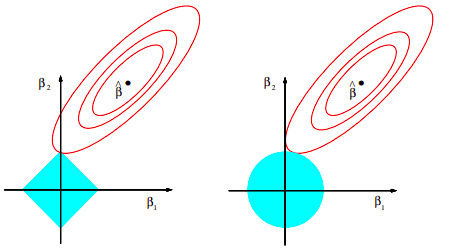
\includegraphics[scale=0.5]{figure/comparacion_regiones.png}
\caption{Regiones de los problemas de optimización, \citep{statisticallearning}}
\end{figure}

\end{frame}

\begin{frame}
\begin{itemize}
    \item Cuando existen predictores altamente correlacionados (linealmente), ridge reduce la influencia de todos ellos a la vez y de forma proporcional, mientras que lasso tiende a seleccionar uno de ellos, dándole todo el peso y excluyendo al resto.
    \item En presencia de correlaciones, esta selección varía mucho con pequeñas perturbaciones (cambios en los datos de entrenamiento), por lo que, las soluciones de lasso, son muy inestables.
\end{itemize}

Para conseguir un equilibrio óptimo entre estas dos propiedades, se puede emplear lo que se conoce como penalización elastic net, que combina ambas estrategias.
\end{frame}

\subsection{Elastic Net}
\begin{frame}{Elastic Net}
 \cite{elastic_net} presentan por primera vez este enfoque de penalización, el cual es una generalización de las penalización \textit{ridge} y \textit{lasso}, llamado \textit{elastic net}. La estimación de \textit{elastic net} se define 
\begin{align}\label{elastic_net_equation}
    \hat{\beta} = \arg \min_{\beta} \{||\y-\X \beta ||^2+\lambda_2||\beta||^2+\lambda_1||\beta||\}
\end{align} 
Sea $\alpha = \lambda_2/(\lambda_1+\lambda2),$ entonces resolver $\hat{\beta}$ en (\ref{elastic_net_equation}) es equivalente a el siguiente problema de optimización
\begin{align}
    \hat{\beta} &= \arg \min_{\beta} \left\{ ||\y-\X\beta||^2 \right\}\\
    s.a. &\ \ \ (1-\alpha)||\beta||+\alpha||\beta||^2\leq t.
\end{align}
\end{frame}

\subsection{Extensión LASSO}
\begin{frame}{Extensión Lasso}

\begin{itemize}
    \item Lasso adaptativo:
    \begin{align}
        \arg \min_{\beta} ||\y-\beta\X||^2+\lambda\sum_{j=1}^p w_j|\beta_j|. 
    \end{align}
    donde $w$ es un vector de pesos conocido \citep{elastic_net}.
    \item Lasso agrupado:
    \begin{align}
        \arg \min_{\beta} ||\y-\sum_{l=1}^L\X_l\beta_l||^2+\lambda\sum_{l=1}^L \sqrt{p_l}||\beta_l||_2. 
    \end{align}
    \citep{group_lasso}
\end{itemize}
 


\end{frame}

\section{Ejemplos numéricos.}
\subsection{Delitos}
\subsection{Contenido de grasa}
\begin{frame}{Ejemplo: Delitos y Contenido de grasa.}
A continuación veremos el efecto que tienen los diferentes tipos de regularización en dos problemas diferentes.
\begin{itemize}
    \item Delitos: tuning y efecto del parametro $\lambda$.
    \item Contenido de grasa: efecto de estandarizar los datos.
\end{itemize}
    \begin{cod}
    Ver example$\_$regularized$\_$linear$\_$regressión.ipynb
    \end{cod}
\end{frame}


\section{Extensión de regularización para el caso multivariado.}
\begin{frame}{Regresión multivariada}
La regresión multivariada es una generalización del modelo de regresión clásico pero considerando $q>1$ variables respuestas. Es decir, sea $\X$ la matriz de las variables independientes $n\times p$, $\Y$ la matriz de las variables independientes $n\times q$ y sea $\E$ la matriz de error aleatorio $n\times q$. Entonces el modelo de regresión multivariada es
\begin{align}
        \Y = \X \B +\E,
\end{align}
donde $\B$ es la matriz de coeficientes de regresión $p\times q$. Si $q=1$ el modelo se simplifica al problema de regresión clásico donde $\B$ es el vector de coeficientes de regresión $p-$dimensional.
\end{frame}

\begin{frame}{Función de verosimilitud.}
La función de verosimilitud logarítmica negativa de ($\B, \Omega$), donde $\Omega = \Sigma^{-1}$ se puede expresar como 
\begin{align} \label{log_verosimilitud}
    g(\B,\Omega) = \tr \left[ \frac{1}{n}(\Y-\X\B)^T(\Y-\X\B)\Omega \right] -\log(\det(\Omega))
\end{align}
Es fácil ver (derivando con respecto a $\B$ e igualando a 0, y simplificando), que el estimador de máxima verosimilitud de $\B$ es 
\begin{align} \label{estimador_B_OLS}
    \hat{\B}^{OLS}=(\X^T\X)^{-1}\X^T\Y.
\end{align}
Lo anterior es equivalente a realizar las estimaciones de $\B$ utilizando mínimos cuadrados ordinarios de forma separada para cada una de las q variables de respuestas y no este implica que no dependan  de $\Omega.$ 

\end{frame}

\begin{frame}
De lo anterior podemos observar dos enfoques distintos cuando se considera una regresión multivariada. Lo primero es considerar que los datos no están correlacionados y el otro enfoque es considerar la matriz de covarianzas de los errores.
\begin{itemize}
    \item REMMAP. El problema de minimización con restricciones propuesto por \citep{remap}, consiste en optimizar
    $$ L(\hat{\B},\X,\Y)=  \underset{\B}{argmin} \{\frac{1}{2} \sum_{k=1}^{q} (\y_{k}-\x \B_{k})^{2} \} + \lambda_1 \sum_{k=1}^{q}|\B_{k}| $$
    
    \item MRCE. \cite{mrce} plantea un procedimiento para construir un estimador de una matriz de coeficientes de regresión multivariada,
    \begin{align}\label{log_verosimilitu_penalizado}
    (\hat{\B}, \hat{\Omega}) = \arg \min_{\B, \Omega} \left\{g(\B, \Omega)+\lambda_1\sum_{j'\neq j} |\omega_{j'j}| +\lambda_2\sum_{j=1}^p\sum_{k=1}^q|b_{jk}|\right\} 
\end{align}
\end{itemize}
\end{frame}
\subsection{Ejemplo. Datos sintéticos}
\begin{frame}{Conjunto de datos}
    \begin{itemize}[<+- | alert@+>]
    \item El conjunto de datos sinteticos fue generado con la función $make_regression()$ de la librería de Scikit-learn. Consideramos diferentes parámetros de la función anterior: $n\_samples (n)=[100,20],\  n\_features(p)=[20,100],$ y $ n\_targets(q)=[2,5]$.
    \item Consideramos partir el conjunto de datos original, en dos conjuntos uno de prueba y otro de entrenamiento.
    \item Además de que nuestro conjunto de datos, consideramos una estandarización debido a los supuestos que se tienen en los modelos.
    \end{itemize}
\end{frame}

\begin{frame}{Primeros conjunto de datos}
    Observando la \textbf{Figura \ref{MSE_1}}, podemos notar que cuando se consideran tamaños de $n<p$ notamos que los mejores predictores son ocupando la metodología de REMMAP.
     \begin{figure}[!htb]
 \minipage{0.5\textwidth}
   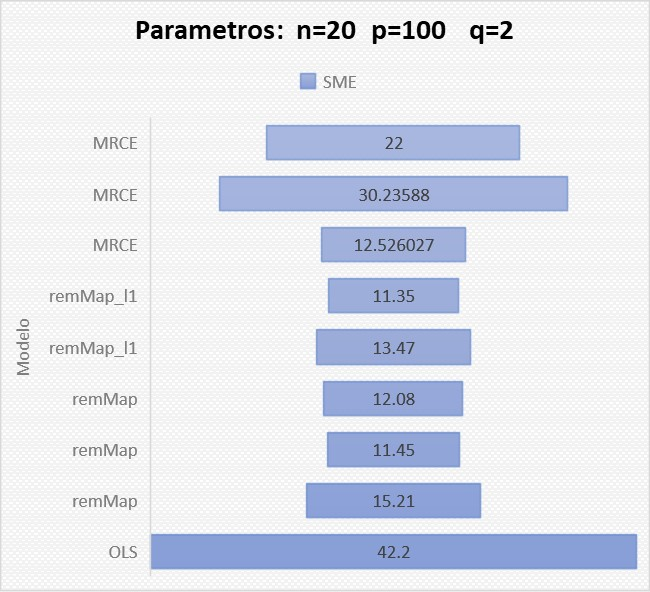
\includegraphics[scale=.4]{figure/im1.jpg}
  \caption{}
 \endminipage
 \minipage{0.5\textwidth}
   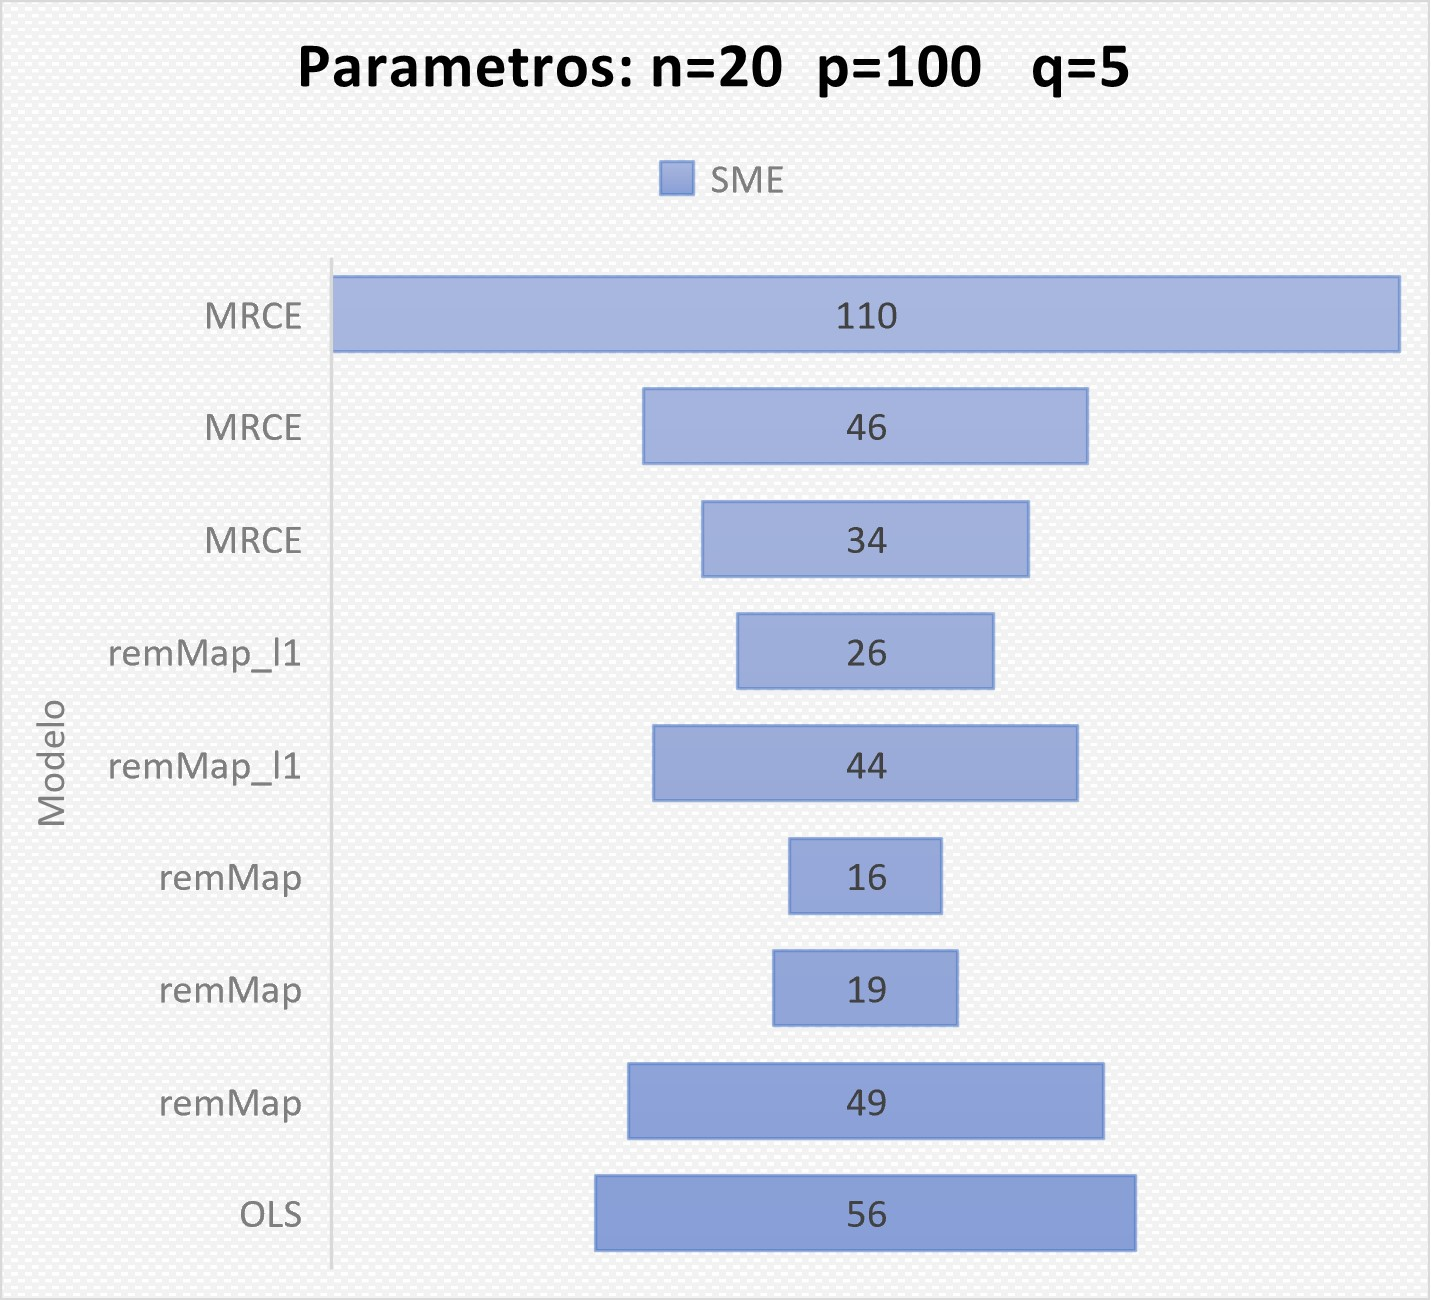
\includegraphics[scale=.4]{figure/im2.jpg}
  \caption{}
 \endminipage
 \caption{MSE considerando distintos modelos, con $n<p.$}\label{MSE_1}
 \end{figure}
\end{frame}

\begin{frame}{$n>p$}
Cuando $n>p$, podemos notar que los estimadores OLS tienen buen rendimiento. Además MRCE tiene rendimientos similares.
 \begin{figure}[!htb]
 \minipage{0.5\textwidth}
   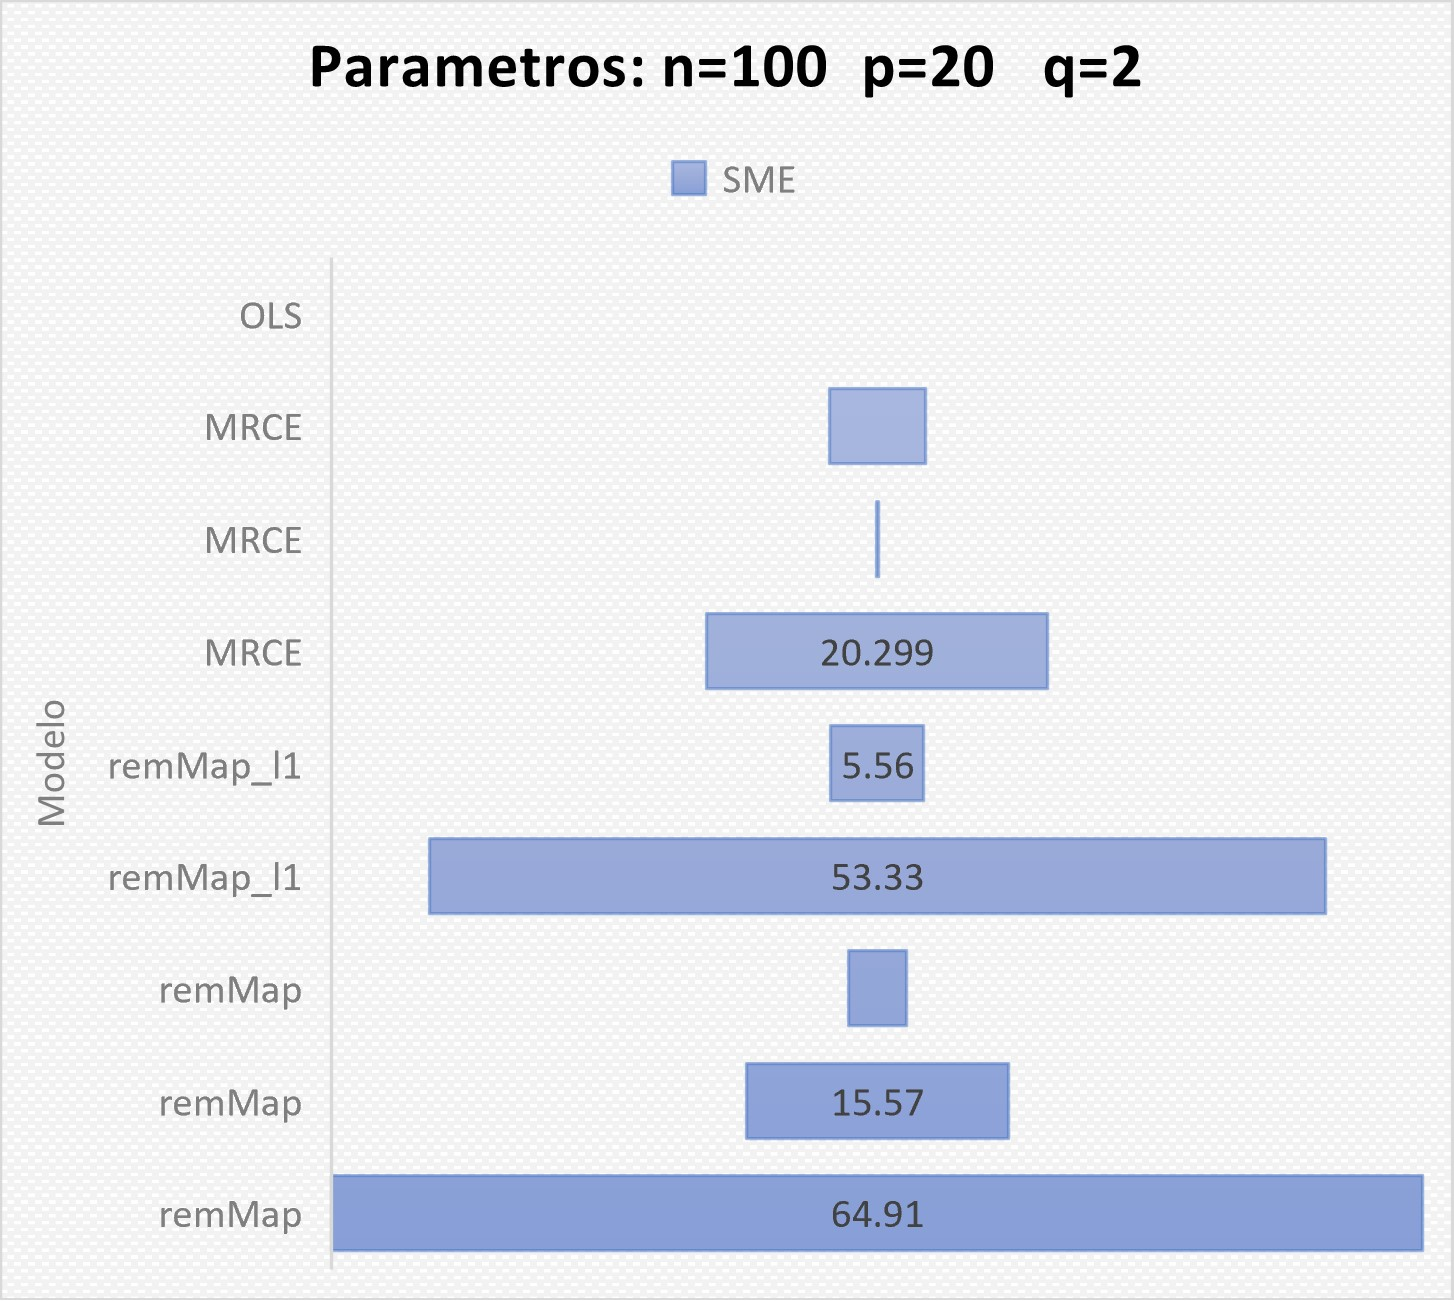
\includegraphics[scale=.4]{figure/im3.jpg}
  \caption{}
 \endminipage
 \minipage{0.5\textwidth}
   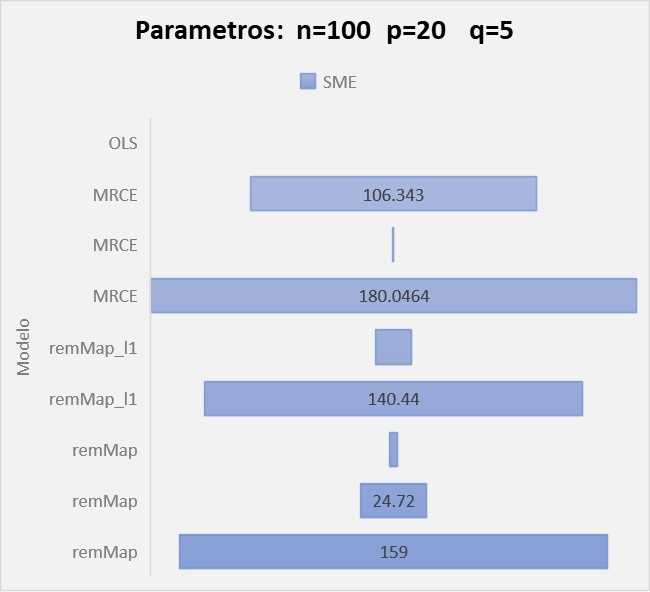
\includegraphics[scale=.4]{figure/im4.jpg}
  \caption{}
 \endminipage
\caption{MSE considerando distintos modelos, con $n>p$.}
 \end{figure}
\end{frame}


\section{Conclusiones}
\begin{frame}
\begin{itemize}[<+- | alert@+>]
    \item Presentamos una alternativa importante cuando los datos incumple los supuestos de mínimos cuadrados. Estas alternativas actualmente son muy usadas en problemas de distintas disciplinas. 
    \item Además este enfoque se puede trasladar a diferentes métodos o modelos, por ejemplo, \cite{cox_lasso} presenta una modificación al modelo de Cox utilizando regularización.  
    \item Resaltamos las diferencias y ventajas que tiene los diferentes tipos de regularización, es decir, como regresión ridge funciona mejor en casos cuando existe multicolinealidad y regresión lasso tiene mejor rendimiento cuando existe un grupo de variables representativas en el modelo. 
\end{itemize}
    
\end{frame}

\printbibliography




\end{document}
